%1. Describe EKS cluster
%2. Describe how was operator installed (screenshots etc)
%3. Describe prepared CRD
%4. Describe execution (screenshots)
%4.1 Aligning
%4.2 Prediction
%4.3 Post Processing
%5. Describe artifacts
%6. Show SMS

\chapter{Methods and Experiments}

Niniejszy rozdział ma za zadanie opisać sposób testowania oprogramowania KubeFold na platformie AWS oraz omówi wyniki obliczeń.


\section{Runtime environment}

Projekt był uruchamiany na platformie AWS EKS~\ref{subsec:aws-eks}.
Do szybkiego uruchomienia klastra użyto narzędzia \texttt{eksctl}, któremu podano konfigurację klastra w regionie \texttt{eu-central-1} z dwiema grupami węzłów-CPU i GPU.
Konfiguracja została przedstawiona na listingu~\ref{lst:eksctl}.
Warto zwrócić uwagę na dołączone polityki AWS IAM dające uprawnienia grupom węzłów do usług takich jak AWS S3, AWS SNS czy też AWS FSx.

\begin{lstlisting}[language=yaml,caption={\texttt{eksctl} configuration used for launching AWS EKS cluster},label={lst:eksctl}]
apiVersion: eksctl.io/v1alpha5
kind: ClusterConfig
metadata:
  name: alphafold-cluster
  region: eu-central-1

managedNodeGroups:
  - name: ng-primary # Cheaper node group without GPU devices
    instanceType: m5.xlarge
    desiredCapacity: 1
    subnets:
      - "subnet-038b10f6f4ac5aacd"
    iam:
      withAddonPolicies:
        ebs: true
        fsx: true
        efs: true
      attachPolicyARNs:
        - arn:aws:iam::aws:policy/AmazonEKSWorkerNodePolicy
        - arn:aws:iam::aws:policy/AmazonEKS_CNI_Policy
        - arn:aws:iam::aws:policy/AmazonFSxFullAccess
        - arn:aws:iam::aws:policy/AmazonS3FullAccess
        - arn:aws:iam::aws:policy/AmazonSNSFullAccess
        - arn:aws:iam::aws:policy/AmazonEC2ContainerRegistryReadOnly
        - arn:aws:iam::aws:policy/AmazonSSMManagedInstanceCore
  - name: ng-gpu # More expensive node group with GPU devices
    instanceType: g5.xlarge
    desiredCapacity: 1
    subnets:
      - "subnet-038b10f6f4ac5aacd"
    iam:
      withAddonPolicies:
        ebs: true
        fsx: true
        efs: true
      attachPolicyARNs:
        - arn:aws:iam::aws:policy/AmazonEKSWorkerNodePolicy
        - arn:aws:iam::aws:policy/AmazonEKS_CNI_Policy
        - arn:aws:iam::aws:policy/AmazonFSxFullAccess
        - arn:aws:iam::aws:policy/AmazonS3FullAccess
        - arn:aws:iam::aws:policy/AmazonSNSFullAccess
        - arn:aws:iam::aws:policy/AmazonEC2ContainerRegistryReadOnly
        - arn:aws:iam::aws:policy/AmazonSSMManagedInstanceCore

iam:
  withOIDC: true
  serviceAccounts:
    - metadata:
        name: fsx-csi-controller-sa
        namespace: kube-system
        labels: { aws-usage: "application" }
      attachPolicyARNs:
        - "arn:aws:iam::aws:policy/AmazonFSxFullAccess"

vpc:
  id: vpc-0ade33da149682ec2
  subnets:
    public:
      eu-central-1a:
        id: "subnet-038b10f6f4ac5aacd"
      eu-central-1b:
        id: "subnet-099b2b55ca156bb7d"

addons:
  - name: vpc-cni
  - name: coredns
  - name: kube-proxy
  - name: eks-pod-identity-agent
\end{lstlisting}

Na klastrze został zainstalowany AWS FSx CSI Driver.
Służy on do automatycznego tworzenia i zarządzania wolumenami AWS FSx for Lustre na postawie utworzonych w klastrze zasobów \texttt{PersistentVolumeClaim}.
By było to możliwe koniecznie jest skonfigurować \texttt{StorageClass}, która wskazuje w jaki sposób powinny być utworzone wolumeny.
W konfiguracji przedstawionej na listingu~\ref{lst:storage-class} ustawiono opcje takie jak wersja systemu plików, typ kompresji (disabled), przepustowość wolumenu oraz opcje sieciowe.
Dzięki temu utworzenie zasobu \texttt{PersistentVolumeClaim} ze wskazaniem na \texttt{StorageClass} o nazwie \texttt{fsx-sc} spowoduje automatycznie provisioning nowego wolumenu w AWS.

\begin{lstlisting}[language=yaml,caption={Definition of \texttt{StorageClass} for FSx CSI Driver},label={lst:storage-class}]
kind: StorageClass
apiVersion: storage.k8s.io/v1
metadata:
  name: fsx-sc
provisioner: fsx.csi.aws.com
parameters:
  subnetId: subnet-038b10f6f4ac5aacd
  securityGroupIds: sg-058c31d84bfd004cf,sg-04e79090b86912eae,sg-07d7ceb3fa050568c,sg-02a2a067c7f724318
  deploymentType: PERSISTENT_1
  perUnitStorageThroughput: "200"
  dataCompressionType: "NONE"
  fileSystemTypeVersion: "2.15"
\end{lstlisting}

Do zainstalowania operatora KubeFold użyto pliku instalacyjnego wygenerowanego przez narzędzie KubeFold.
Znajduje się on w repozytorium kodu w serwisie GitHub w ścieżce \texttt{dist/install.yaml}.
Instalacja zatem sprowadza się do wykonania jednego polecenia: \texttt{kubectl apply -f https://raw.githubusercontent.com/kubefold/operator/ \n refs/heads/main/dist/install.yaml}.
Dzięki temu jest ona bardzo szybka i wygodna z perspektywy administratora.

\begin{lstlisting}[language=bash,caption={Quick project startup script},label={lst:up-script}]
#!/bin/bash

export AWS_PAGER=""
ACCOUNT_ID=$(aws sts get-caller-identity --query Account --output text)
eksctl create cluster -f eks/cluster.yaml
aws eks update-kubeconfig --name alphafold-cluster --region eu-central-1
kubectl config use-context arn:aws:eks:eu-central-1:"$ACCOUNT_ID":cluster/alphafold-cluster
kubectl apply -k "github.com/kubernetes-sigs/aws-fsx-csi-driver/deploy/kubernetes/overlays/stable/?ref=release-1.3"
kubectl apply -f eks/fsx.storageclass.k8s.yaml

kubectl apply -f https://raw.githubusercontent.com/kubefold/operator/refs/heads/main/dist/install.yaml
kubectl apply -f config/samples/data_v1_proteindatabase.yaml

echo 'Done'
\end{lstlisting}

W celu szybkiego postawienia klastra wraz ze wszystkimi potrzebnymi zależnościami został przygotowany skrypt \texttt{up.sh}, który został przedstawiony na listingu~\ref{lst:up-script}.
Po wykonaniu skryptu można bezpośrednio przejść do rozpoczęcia pracy z KubeFold.
Jeżeli klaster został zainstalowany poprawnie, wykonanie polecenia \texttt{kubectl get pods -A} powinno pokazać wyjście podobne do tego na zrzucie ekranu~\ref{fig:eks_pods_terminal}.

\begin{figure}[htbp]
  \centering
  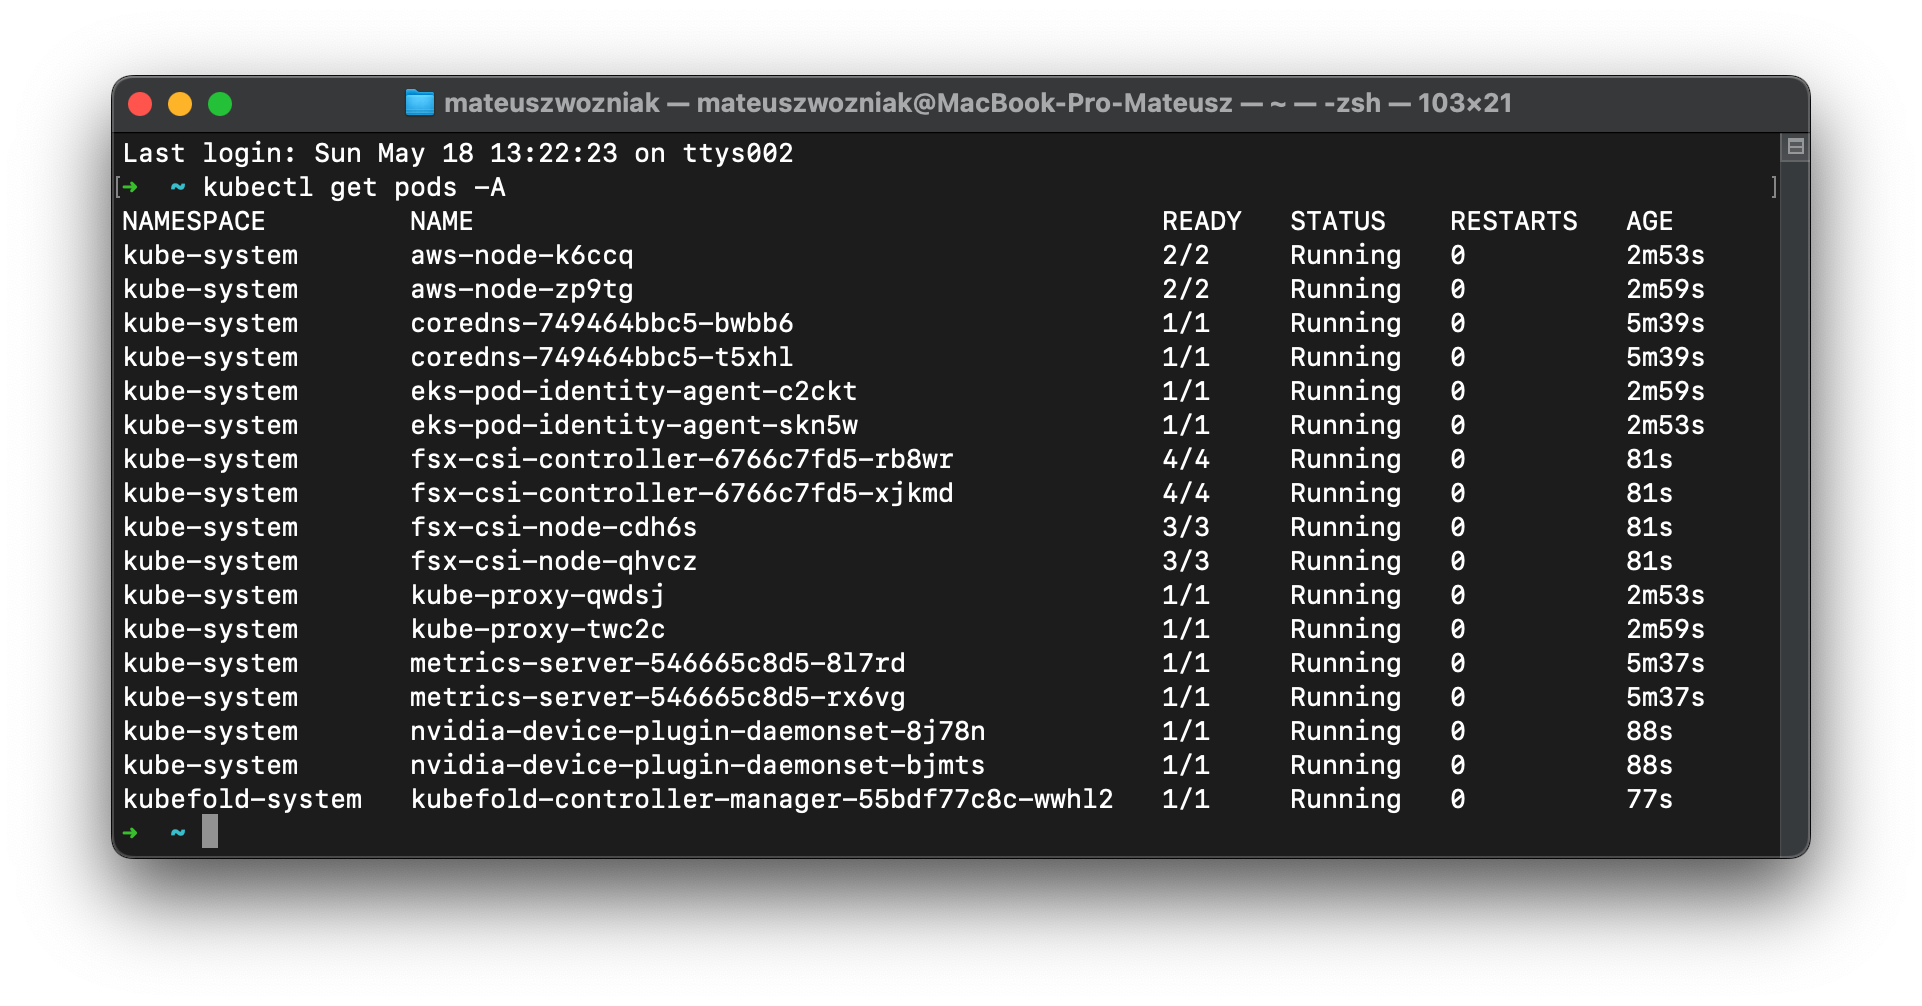
\includegraphics[width=\textwidth]{images/eks_pods_terminal}
  \caption{\texttt{kubectl get pods} output after successful cluster installation}
  \label{fig:eks_pods_terminal}
\end{figure}


\section{Prepared resource definitions}

W celu przeprowadzenia testów KubeFold przygotowano następujące definicje zasobów w kodzie YAML.
Pierwszy z nich to zasób \texttt{ProteinDatabase} przedstawiony na listingu~\ref{lst:used_protein_database}.
Drugi z nich z kolei to zasób \texttt{ProteinConformationPrediction} przedstawiony na listingu~\ref{lst:used_protein_conformation_prediction}.
Oba te zasoby zostały zaaplikowane na klaster za pomocą \texttt{kubectl apply} tuż po instalacji.

\begin{lstlisting}[language=yaml,caption={Used \texttt{ProteinDatabase} resource definition},label={lst:used_protein_database}]
apiVersion: data.kubefold.io/v1
kind: ProteinDatabase
metadata:
  name: proteindatabase-sample
spec:
  datasets:
    bfd: true
    mgyclusters: true
    nt: true
    pdb: true
    pdbseqreq: true
    rfam: true
    rnacentral: true
    uniref90: true
    uniprot: true
  volume:
    storageClassName: fsx-sc
\end{lstlisting}

\begin{lstlisting}[language=yaml,caption={Used \texttt{ProteinConformationPrediction} resource definition},label={lst:used_protein_conformation_prediction}]
apiVersion: data.kubefold.io/v1
kind: ProteinConformationPrediction
metadata:
  name: proteinconformationprediction-sample
spec:
  database: proteindatabase-sample
  protein:
    id: [ 'A','B' ]
    sequence: GMRESY...LQQANDLKQG
  model:
    volume:
      storageClassName: fsx-sc
    weights:
      http: https://staticfilehosting.com/af3.bin.zst
    seeds:
      - 1
  destination:
    s3:
      bucket: kubefold-artifacts-sample
      region: eu-central-1
  notify:
    region: eu-central-1
    sms:
      - "+48140690323"
\end{lstlisting}.

Po utworzeniu zasobu \texttt{ProteinDatabase} FSx CSI Driver spowodował utworzenie systemu plików FSx for Lustre (zobacz rys.~\ref{fig:fsx_fs}).
Gdy tylko system plików został utworzony, proces pobierania baz danych białek rozpoczął się w wielu podach jednocześnie.
Użytkownik może na bieżąco kontrolować postęp pobierania co zostało pokazane na zrzucie ekranu~\ref{fig:used_proteindatabase_terminal}.
Po zakończeniu pobierania status zostanie zmieniony na \textit{Completed} (zobacz zrzut ekranu~\ref{fig:proteindatabase_completed_terminal}).

\begin{figure}[htbp]
  \centering
  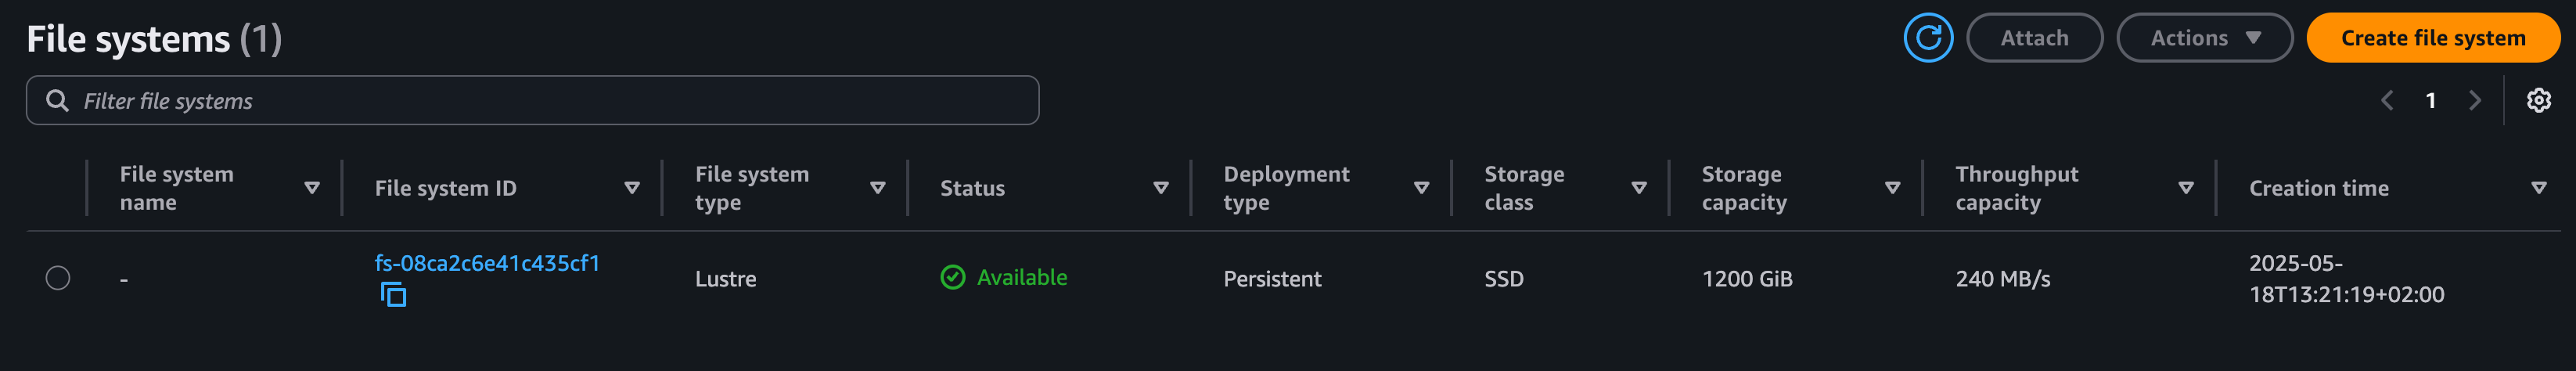
\includegraphics[width=\textwidth]{images/fsx_fs}
  \caption{Created FSx for Lustre file system in AWS Web Console}
  \label{fig:fsx_fs}
\end{figure}

\begin{figure}[htbp]
  \centering
  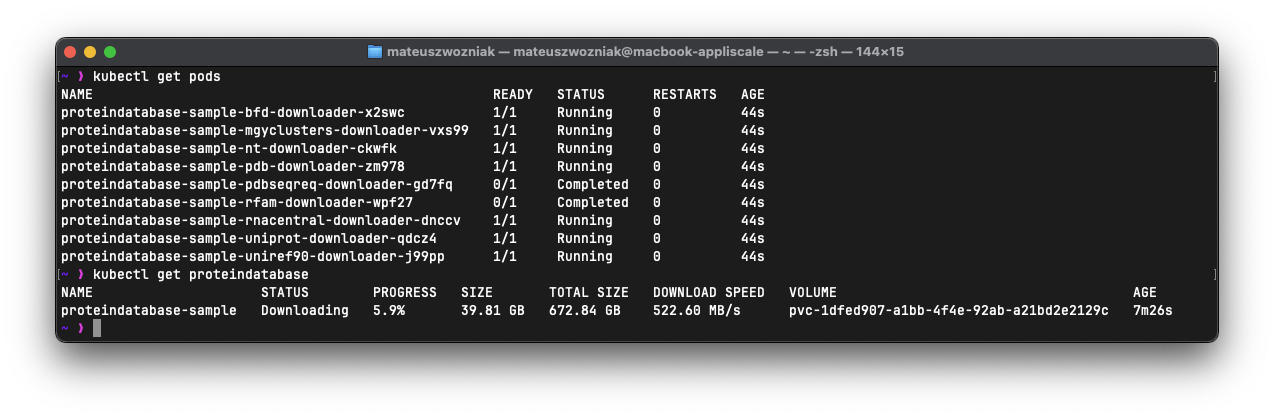
\includegraphics[width=\textwidth]{images/old_proteindatabase_terminal}
  \caption{Terminal output presenting \texttt{ProteinDatabase} resource}
  \label{fig:used_proteindatabase_terminal}
\end{figure}

\begin{figure}[htbp]
  \centering
  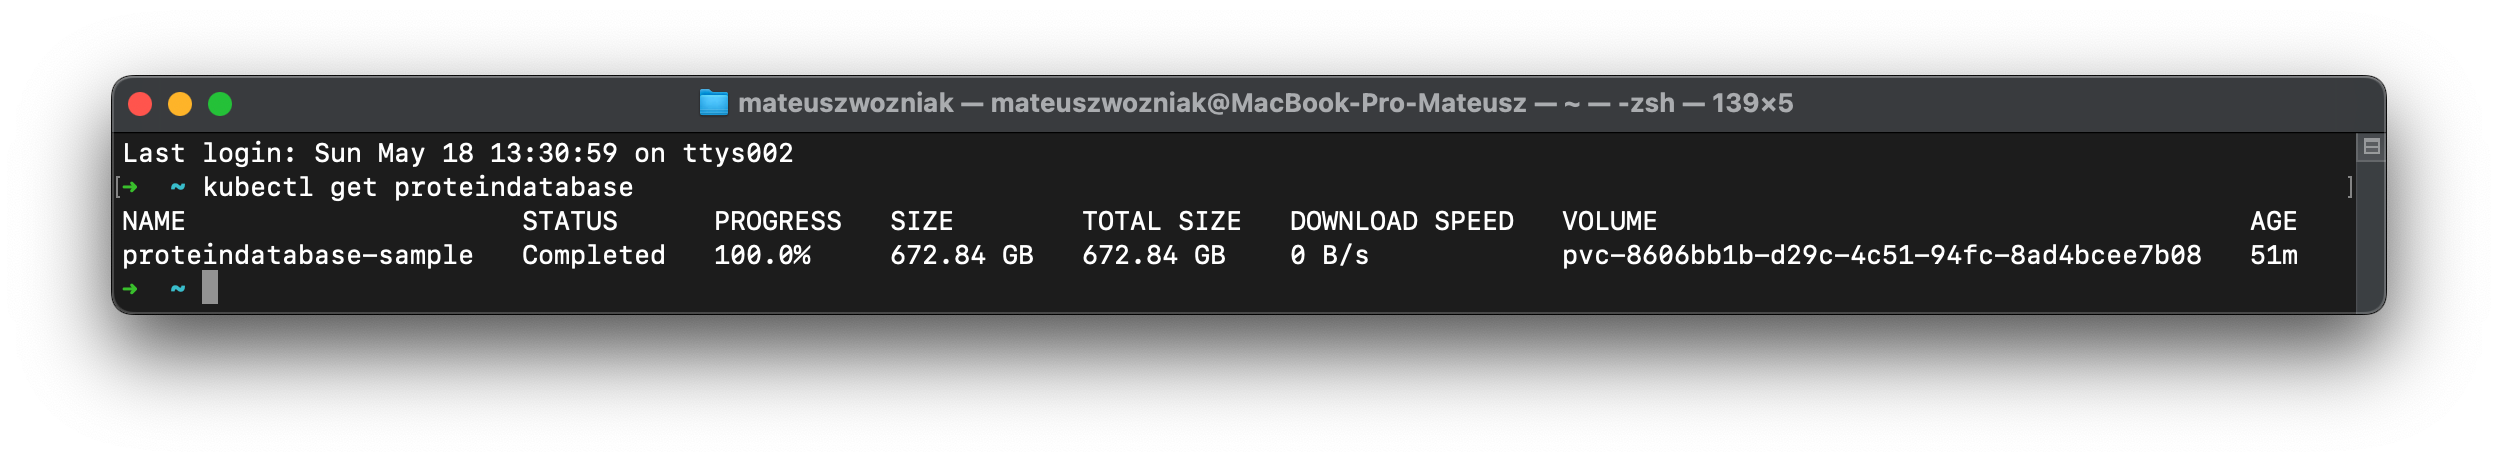
\includegraphics[width=\textwidth]{images/proteindatabase_completed_terminal}
  \caption{Completed downloading of protein database}
  \label{fig:proteindatabase_completed_terminal}
\end{figure}

\section{Computation artifacts overview}